% This template was originally by R. Jacob Vogelstein
% Updated on March 1, 2010 by Noah J. Cowan

% Brian began working on thesis on February 2, 2017

\documentclass[12pt,oneside,final]{thesis}

\usepackage[superscript]{cite}
\usepackage{amsmath,amsfonts}
\usepackage{graphicx}
\graphicspath{{./figs/}}
\usepackage{fixltx2e}
\usepackage{array}
% wrapfig is fragile: use sparingly
\usepackage{wrapfig} 
%\usepackage{times}  % Use this for ugly fonts

\usepackage{upgreek}
\usepackage{hyperref}
\usepackage{setspace}

\usepackage{booktabs}
\usepackage{multirow}
\usepackage{longtable}
\usepackage[font=singlespacing, labelfont=bf]{caption}
%\usepackage{CV}

\usepackage{enumitem}
\newlist{inlinelist}{enumerate*}{1}
\setlist*[inlinelist,1]{%
  label=(\arabic*),
}

\usepackage{fancyhdr}    % Use nice looking headers along with the required footer page numbers   
%\usepackage[hypertex]{hyperref}

%Define the header/footer style
\pagestyle{fancy}
\fancyhf{}
\setlength{\headheight}{15pt}
\lhead{\leftmark}
\cfoot{\thepage}
\renewcommand{\headrulewidth}{0pt}
\fancypagestyle{plain}{% Redefine ``plain'' style for chapter boundaries
\fancyhf{} % clear all header and footer fields
\fancyfoot[C]{\thepage} % except the center
\renewcommand{\headrulewidth}{0pt}
\renewcommand{\footrulewidth}{0pt}}

%\tolerance=10000

%\makeglossary % enable the glossary

\begin{document}

\title{Grouping mechanisms for object-based vision and attention}
\author{Brian H. Hu}
\degreemonth{May}
\degreeyear{2017} 
\dissertation
\doctorphilosophy
\copyrightnotice


% add your chapters, best way is to have separate TeX files for each chapter
%% FRONTMATTER
\begin{frontmatter}

% generate title
\maketitle

\begin{abstract}

Abstract goes here.

\vspace{1cm}

\noindent Primary Reader: Ernst Niebur\\
Secondary Reader: R{\"u}diger von der Heydt

\end{abstract}

\begin{acknowledgment}

As I was sitting on the boat, I was thinking about how the trip was really a metaphor for my PhD experience. I have had opportunities to steer the boat (sometimes in the wrong direction!), gone through both good and bad weather, and through it all, have had a good captain whom I can trust to guide me though the finish. Best,

\end{acknowledgment}

\begin{dedication}
 
This thesis is dedicated to \ldots

\end{dedication}

% generate table of contents
\tableofcontents

% generate list of tables
\listoftables

% generate list of figures
\listoffigures

\end{frontmatter}

\chapter{Introduction}
\label{sec:intro}
\chaptermark{Introduction}

%Introduction.

\section{Segmentation and figure-ground organization}
The task of partitioning an image into regions bounded by contours (segmentation) and the task of assigning border-ownership of these contours to either the foreground or the background (figure-ground organization) are important first steps in achieving image understanding. Gestalt psychologists were the first to recognize the importance of the whole in influencing perception of the parts, and with this observation, laid out several principles for figure-ground organization~\citep{Koffka35, Wertheimer23}. For example, the rule of good continuation states that well-aligned contour elements should be grouped together. This is closely related to the concept of a ''local association field,'' where collinear contour elements excite each other and noncollinear elements inhibit each other~\citep{Ullman92, Field_etal93}. Results from neuroanatomy lend support to these ideas, as the lateral connections within V1 predominantly link similar-orientation cortical columns. However, our understanding of the neural mechanisms of these processes remains surprisingly limited.
 
The brain must keep track of which regions and contours belong to which objects. This is known as the binding problem, as it is not clear how the features of an object are bound together~\citep{Treisman96b}. One class of models relies on the fast temporal coding structures of spike trains \citep{Singer99b}, but experimental evidence is controversial~\citep{Thiele_Stoner03,Roelfsema_etal04,Dong_etal08a}. Another solution involves differential neural activity, where the neurons responding to the features of an object show increased firing compared with neurons responding to the background. This response enhancement is known as figure-ground modulation (FGM), and was first observed in primary visual cortex (V1) for texture-defined figures~\citep{Lamme95}. Similar results have been found using other tasks and techniques, including more recent voltage-sensitive dye imaging of populations of neurons during a contour grouping task~\citep{Gilad_etal13}. However, this solution only works if there is a single object in the foreground, as multiple objects each labeled with higher neural activity could be interpreted as parts of a single object. Furthermore, each neuron's firing rate is inherently ambiguous, as higher activity could be due to labeling with FGM or because the neuron's preferred feature falls within its receptive field. As a result, the binding problem cannot be solved with models that only represent object information in terms of enhanced neural activity in early visual areas~\citep{Niebur00a}. This strongly points to neural circuits that employ populations of neurons which explicitly represent (\ie in their firing rate) the organization of the visual scene in terms of perceptual objects.

\section{The role of cortical feedback}
\comment{The resulting computational model developed by~ \citet{Stemmler_etal95b} has since been corroborated by a large number of independent studies~\citep[e.g.][]{Simonotto_etal97,Polat_etal98,Chatterjee_etal11,Xie_etal14}.}
%
Early computational models~\citep{Stemmler_etal95b} and experimental studies~\citep{Simonotto_etal97,Polat_etal98,Chatterjee_etal11,Xie_etal14} put forth the view that horizontal connections
% However, in agreement with others at the time, the underlying concept of horizontal connections in that model was that they
are essentially static, or varying over time scales given by ontogenetic development or neuronal plasticity. Such structures could thus implement overall statistics of natural scenes~\citep[like circular structures, e.g.][]{Sigman_etal01} but they could not flexibly represent the myriad of instantaneously present and constantly changing visual shapes observed during perception of dynamic scenes. This view has been considerably enlarged over the last decade or so, and what is emerging is a view in which the lateral connections are in place but can be actively and rapidly modulated by top-down connectivity from higher areas.

The degree of collinear facilitation observed in V1 is strongly context-dependent, and can change with the behavioral task~\citep{Li_etal04, Li_etal06} as well as perceptual learning~\citep{Li_etal08a, Yan_etal14}. As a result, feedback connections from higher areas may play an important role in shaping the responses of neurons in early visual areas. In fact, simultaneous neural recordings from areas V1 and V4 during two different figure-ground segregation tasks show that V4 is intimately involved in the FGM process~\citep{Poort_etal12, Chen_etal14}. In these studies, the FGM signal appears first in V4 and is then fed back to V1, with a delay representing recurrent processing. Additional studies of curve-tracing~\citep{Roelfsema_etal98} and border-ownership~\citep{Zhou_etal00, Qiu_etal07, Zhang_vonderHeydt10} further demonstrate that feedback mechanisms are necessary for explaining FGM in the presence of multiple objects. However, essential questions still remain about the nature of the interactions between and within different cortical areas. How is early-level feature information about an object combined with global context information about the object in a synergistic way in order to generate FGM?

\section{The role of attention}
Behavioral studies have shown that attention can be directed to objects~\citep{Egly_etal94} and electrophysiological results demonstrate that attention can act as a top-down signal which influences FGM~\citep{Qiu_etal07, Poort_etal12}. In an ambiguous figure-ground display, attending to one region increases the probability that this region is perceived as figure~\citep{Driver_Baylis96, Vecera_etal04}. Spatial attention, which has been extensively studied, acts like a ''spotlight'' that enhances neural responses within the focus of attention and suppresses responses outside~\citep{Motter93a}. Attention can also operate in a feature-based or object-based manner. Feature-based attention acts broadly across the visual scene and increases the responses of all components that share similar feature attributes (e.g. color, orientation, or direction of movement) with the attended component~\citep{Treue_Trujillo99}. Object-based attention highlights all the parts of an object, also encompassing all the features that belong to the object~\citep{Roelfsema_etal98, Schoenfeld_etal14}. Attention has been found to modulate border-ownership in an object-based manner~\citep{Qiu_etal07}. Border-ownership is a property of many neurons in V2 which encodes the side to which an object border
belongs relative to their receptive field \citep{Zhou_etal00}. To explain these results,~\citet{Craft_etal07} proposed a model in which populations of grouping neurons explicitly represent (in their firing rates) the perceptual organization of the visual scene. Grouping neurons are reciprocally connected to border ownership selective (BOS) neurons through feedforward and feedback connections. Attention broadly targets grouping neurons, which can then modulate the activity of BOS neurons through feedback~\citep{Mihalas_etal11b}. A feedforward version of this model has been applied to natural images, where it outperforms other models in predicting the location of eye fixations~\citep{Russell_etal14}.

\section{Grouping of 3D surfaces}
Grouping mechanisms are important not only for piecing together object contours, but also for providing a structure for selectively attending
to groups of objects~\citep{Treisman_Gelade80}. Supported by extensive psychophysical data,~\citet*{Nakayama_etal95} proposed that surface
representations play a key role in intermediate-level vision. For example, by selectively attending to a surface in 3D space, subjects can perform efficient search for a conjunction target~\citep{Nakayama_Silverman86}. In a separate cueing experiment, attention was shown to spread automatically across surfaces~\citep{He_Nakayama95}. These abilities indicate powerful mechanisms for grouping objects into surfaces in 3D space, and suggest that structuring the world in terms of surfaces might be an ecologically important function (\eg for locomotion along the ground
plane, reaching for objects along a table top \etc). The use of basis functions provides a suitable theoretical framework for understanding how multiple surfaces can be efficiently represented in the same population of neurons. Modeling the grouping of 3D surfaces will provide insight into the neural circuits that represent surfaces, filling a critical gap in our understanding of intermediate-level vision.

\section{Overview of the grouping model}
\begin{figure}[t]
\centering
\includegraphics[width=0.75\textwidth]{Intro/figs/groupingcircuit}
\makeatletter
\let\@currsize\normalsize
\caption{Overview of the grouping model}
\label{fig:GroupingModel}
\end{figure}

Several models have been proposed~\citep{Zhaoping05, Sakai_Nishimura06,Craft_etal07, Layton_etal12} to describe how a neuron's border ownership selectivity can be modulated by visual input far away from its classical receptive field (RF). In the grouping model~\citep{Craft_etal07}, BOS neurons participate in neural circuits that define perceptual objects early-on in processing (Figure~\ref{fig:GroupingModel}). An object border activates a pair of orientation-selective BOS neurons whose RFs are shown as ellipses. The arrows on the RFs point towards the preferred direction of the neuron, indicating where the object is relative to the neuron's RF. BOS neurons activated by the solid-line square (red ellipses) excite the appropriate grouping neuron (red G in circle) through feedforward connections (red solid lines). The grouping neuron in turn enhances the activity of the same BOS neurons through feedback connections (red dotted lines). This type of facilitatory feedback may be mediated by NMDAR channels, which allow gating of sensory input by top-down signals~\citep{Palmer_etal14}. Neurons consistent with other objects (e.g. the dashed-line square) project to other grouping neurons (blue G in circle in this case). Presence of the solid-line square increases the firing rate of the red grouping neuron over that of the blue (and other) grouping neurons since the latter receive less feedforward input. As a consequence, the red grouping neuron provides more feedback to the red BOS neurons than the blue and gray BOS neurons would receive from their respective grouping neurons. Likewise, presence of the dashed-line square increases the firing rates of all blue neurons over those of gray and red neurons. Thus, an object border is represented by two BOS neurons whose relative activity codes for the side of ownership. The relative difference in firing rate is also known as the BOS signal~\citep{Zhou_etal00}.

The BOS signal appears \textasciitilde 25 ms after the visual response to an oriented edge, and the delay is essentially independent of object size \citep{Zhou_etal00}. This constant delay is consistent with a model in which grouping neurons of different sizes integrate local edge signals, and by feedback enhance the same edge  signals~\citep{Craft_etal07}. Attention enhances a BOS neuron's response when an object is on the neuron's preferred side, but has a suppressive effect if the object is on the non-preferred side~\citep{Qiu_etal07}. This asymmetry is consistent with a model in which top-down attention targets grouping neurons, which then modulate the activity of BOS neurons through feedback~\citep{Mihalas_etal11b}. Additional support for the grouping model comes from observations of short-term memory of BOS signals~\citep{OHerron_vonderHeydt09} and remapping of BOS signals across saccades and object movements~\citep{OHerron_vonderHeydt13}. These findings are difficult to explain with models that only represent object information in terms of neural activity in early visual areas. I believe that this strongly points to neural circuits that employ populations of neurons which explicitly represent (\ie in their firing rate) the organization of the visual scene.

\section{Summary of thesis}
The work presented in this thesis deepens and extends our understanding of the neural mechanisms of FGM. In Chapter 1, we introduce background information needed to understand the physiology and previous modeling experiments. In Chapter 2, we propose a quantitative neural model of grouping constrained by physiological data. We validate the model by reproducing several experimental results related to contour integration and border-ownership assignment. In Chapter 3, we extend this model to natural scenes, and our model results are quantitatively compared with both experimental results and human-annotated figure-ground labels (Berkeley Segmentation Dataset). Beginning with Chapter 4, we shift our focus to the representation of 3D information in the visual system. First, we show that a grouping model can reproduce results from a set of psychophysical experiments where attention had to be directed to surfaces. We then show that 3D surfaces can be represented by a feedforward, linear combination of basis functions whose response properties are similar to those of disparity-selective neurons commonly found in early visual cortex. In Chapter 5, we propose a model of 3D visual saliency and show that the added depth information improves saliency prediction.

%%% Local Variables:
%%% mode: latex
%%% TeX-master: "../root"
%%% End:


%\appendix

\chapter{Grouping Model Network}
\label{sec:appendix}
\chaptermark{Grouping Model Network}

\section{Details of model implementation}
\label{sec:appendix_eq}

One pixel in our model input represents the typical size of the receptive
field for 
a V1
edge cell (which at eccentricity 5 $\deg$ is about 0.7
$\deg$, Chen {\em et al}. 2014).  The simulated visual field is
assumed to be homogeneous
(\ie, we neglect the influence of the cortical magnification factor).  
To avoid unbalanced inputs near the
boundaries of the visual field we use periodic boundary
conditions. Each neuronal unit in the model represents multiple
neurons with overlapping receptive fields and similar tuning.  It is
referred to as a ``neuron'' in the following and it is represented by
an ordinary differential equation, eq.~1.  For all examples the system
is simulated for 0.5s and an equilibrium is reached within a few tens
or about hundred ms.  A typical simulation of a visual field of
$64\times 64$ units consists of 30,528 coupled ordinary differential
equations which are solved using a fourth-order Runge-Kutta  algorithm
in MATLAB.

Each neuron is characterized by its spatial location, its type (edge
cell, object grouping cell, \etc) and one additional property, as
follows. E cells are indexed by the angle of their preferred
orientation: $0$, $\pi/4$, $\pi/2$, and $3\pi/4$
(all angles relative to the horizontal). 
B cells are indexed
by the angle of their preferred side of figure: right, $0$; upper
right, $\pi/4$; up, $\pi/2$; upper left, $3\pi/4$; left, $\pi$; lower
left, $5\pi/4$; down, $3\pi/2$; lower right, $7\pi/4$. 
Note that the preferred side of a 
B~cell
 is always orthogonal to its preferred orientation. Contour
grouping cells are indexed by their preferred orientation ($0$,
$\pi/4$, $\pi/2$, and $3\pi/4$), while object grouping neurons are
selective for annuli of a preferred radius.
As discussed earlier, we only use one preferred radius in this model,
which we chose as corresponding to 16 pixels in the input layer.
The network receives two types
of inputs. A binary edge map activates E~cells, taking value 1 if an
edge of that orientation is present
at this location in the image and (-1)
otherwise. Finally, an attentional field stimulates grouping cells,
with maximal strength of 0.07. This value is listed in
Table~\ref{partable}, as are those of all other model parameters.

In the following, we define the anatomical connection patterns between
all neuronal populations in our model. Obviously, this defines the
receptive (and projective) fields of all model neurons. At the input
level, edge cells ($E$ population)  receive 
one-to-one
connections from input units
($IN$ population) of the respective preferred
orientations $o_i$ at 
position $(x,y)$,
resulting in
a connectivity weight distribution as follows,
\begin{align}
	WIN^{o_1}_{x,y}E^{o_2}_{x,y}=
	\begin{cases}
	intoe_w \:\;&if\;o_1 = o_2\\\nonumber
	-1\;&otherwise
	\end{cases}\\
\end{align}
where the weight of the input to edge cell connections, $intoe_w$ is a
scaling parameter, and its value is set to 1.  Changing it does not
produce different activation patterns in the network but rather scales
up all activities.

The connections from edge cells 
to inhibitory IE cells are two-dimensional isotropic Gaussians: 

\begin{align}
	&WE_{x_1,y_1}IE_{x_2,y_2}=N_{etoie}\: \exp\left(-\frac{(x_1-x_2)^2}{2\: etoie_{sd}^2}-\frac{(y_1-y_2)^2}{2\: etoie_{sd}^2}\right)\
\end{align}
where the normalization coefficient $N_{etoie}$ is determined from:
\begin{align}
	etoie_w = \sum^{24}_{i,j=-24} WE_{x,y}IE_{x+i,y+j}
\label{eq:normalizationetoie}
\end{align}

The weight of the edge to IE connections $etoie_w$ is set to 8. The standard deviation of the lateral connections,
$etoie_{sd}$ was chosen to be eight times the size of the edge cells'
receptive field size. For simplicity, all lateral connections in V1
are assumed to have the same standard deviation.
The upper limit in the sum of eq.~\ref{eq:normalizationetoie} is where
we truncate the Gaussian distribution used to define the
connectivities, at three times its standard deviation (8), equal to 24
times the size of a V1 RF.

IE cells are not orientation selective, and inhibit all edge cells in
their neighborhood. The strength of inhibition is independent of
the preferred orientation of the edge cells and has the same
pattern as the reciprocal edge to IE cell connections: 
\begin{align}
	&WIE_{x_1,y_1}E_{x_2,y_2}=N_{ietoe}\: \exp\left(-\frac{(x_1-x_2)^2}{2\: ietoe_{sd}^2}-\frac{(y_1-y_2)^2}{2\: ietoe_{sd}^2}\right)\
\end{align}
where the normalization coefficient $N_{ietoe}$ is determined from:
\begin{align}
	ietoe_w = \sum^{24}_{i,j=-24} WIE_{x,y}E_{x+i,y+j}
\end{align}

The strength of the inhibitory connections IE to edge cells,
$ietoe_w$, is an important parameter in the model. Its value was
chosen to be -8, which is just strong enough for the inhibition of the
edge cells to cancel out activity in the case of a uniform stimulation
field. In our model, attention in the absence of edges is a broad
field, and experimental observations show little effect of attention
alone on the firing rates of purely sensory (edge) cells.
E cells locally connect to other edge cells of the same preferred
orientation. These connections allow for the passing of contour
information along a line. The connection weights are,
\begin{align}
	WE^{o_1}_{x_1,y_1}E^{o_2}_{x_2,y_2}&=N_{etoe}\: \delta_{o_1,o_2}\: \delta_{y_1,0}\: \delta_{y_2,0}\:
	\exp\left(-\frac{(x_1-x_2)^2}{2\: etoe_{sd} ^2}\right)\ {\rm
          if}\ o_1,o_2 = 0 \nonumber\\
	WE^{o_1}_{x_1,y_1}E^{o_2}_{x_2,y_2}&=N_{etoe}\: \delta_{o_1,o_2}\: \delta_{x_1,y_1}\: \delta_{x_2,y_2}\: 
	\exp\left(-\frac{(x_1-x_2)^2}{2\: etoe_{sd} ^2}\right)\  {\rm
          if}\ o_1,o_2 = \pi/4 \nonumber\\
	WE^{o_1}_{x_1,y_1}E^{o_2}_{x_2,y_2}&=N_{etoe}\: \delta_{o_1,o_2}\: \delta_{x_1,0}\: \delta_{x_2,0}\:
	\exp\left(-\frac{(y_1-y_2)^2}{2\: etoe_{sd} ^2}\right)\  {\rm
          if}\ o_1,o_2 = \pi/2 \nonumber\\
	WE^{o_1}_{x_1,y_1}E^{o_2}_{x_2,y_2}&=N_{etoe}\: \delta_{o_1,o_2}\: \delta_{x_1,-y_1}\: \delta_{x_2,-y_2}\: 
	\exp\left(-\frac{(y_1-y_2)^2}{2\: etoe_{sd} ^2}\right)\  {\rm
          if}\ o_1,o_2 = 3\pi/4 \nonumber\\
\end{align}
where the normalization coefficient $N_{etoe}$ is determined from:
\begin{align}
	etoe_w = \sum^{24}_{i,j=-24} WE^{o}_{x,y}E^{o}_{x+i,y+j}
\end{align}

The weight of the excitatory lateral connections $etoe_w=2/3$ is
chosen such that individual excitatory connections are stronger than
the nonspecific inhibitory connections for a line of cells along the
preferred direction, 
and that the integral of the excitatory connections is smaller than
the integral of the inhibitory ones. The standard deviation
$etoe_{sd}=8$ is the same as for all other lateral connections in V1.  

The edge cells E excite a pair of border-ownership cells with the same
preferred orientation $o_1$
and at the same position, $(x_i,y_i)$.  Border ownership selective
cells have opposite 
side-of-figure preferences
$o_2$ which are orthogonal to $o_1$
(\ie differing by $\pi/2$ in either direction).
They are generated by
connections from E cells whose  weight is given by  a 2D Gaussian, 
\begin{align}
	WE^{o_1}_{x_1,y_1}B^{o_2}_{x_2,y_2}&=etob_w \:	\exp\left(-\frac{(x_1-x_2)^2}{2\: etob_{sd} ^2}-\frac{(y_1-y_2)^2}{2\: etob_{sd} ^2}\right)\ \nonumber\\
	%&\sin^2(o_1-o_2) = 1 \nonumber\\
	o_1&\in \left\{0,\pi/4,\pi/2,3\pi/4 \right\} \nonumber\\
	o_2&\in \left\{0,\pi/4,\pi/2,3\pi/4,\pi,5\pi/4,3\pi/2,7\pi/4\ \right\} \nonumber\\
\end{align}
where the weight of the E to border-ownership connections, $etob_w$ is set to 1.

The connections from border-ownership to inhibitory IB cells are two-dimensional Gaussians: 
\begin{align}
	&WB_{x_1,y_1}IB_{x_2,y_2}=N_{btoib}\: \exp\left(-\frac{(x_1-x_2)^2}{2\: btoib_{sd}^2}-\frac{(y_1-y_2)^2}{2\: btoib_{sd}^2}\right)\
\end{align}
where the normalization coefficient $N_{btoib}$ is determined from:
\begin{align}
	btoib_w = \sum^{12}_{i,j=-12} WB_{x,y}IB_{x+i,y+j}
\end{align}

The weight of the border-ownership to IB connections $btoib_w$ is set to 2. The standard deviation of the lateral connections,
$btoib_{sd}$ was chosen to be four times the size of the border-ownership cells' receptive field size. For simplicity, all lateral connections in V2 are assumed to have the same standard deviation.

IB cells, which are not orientation selective, inhibit all border-ownership in their neighborhood with the same pattern as B to IB cell excitation:
\begin{align}
	&WIB_{x_1,y_1}B_{x_2,y_2}=N_{ibtob}\: \exp\left(-\frac{(x_1-x_2)^2}{2\: ibtob_{sd}^2}-\frac{(y_1-y_2)^2}{2\: ibtob_{sd}^2}\right)\
\end{align}
where the normalization coefficients $N_{ibtob}$ is determined from:
\begin{align}
	ibtob_w = \sum^{12}_{i,j=-12} WIB_{x,y}B_{x+i,y+j}
\end{align}

The strength of the inhibitory connections IB to border-ownership, $ibtob_w$, is an important parameter in the
model. Its value was chosen to be -2, which is just strong enough for
the inhibition of the border-ownership cells to 
cancel out activity
in the case of a uniform stimulation field. In our model, attention in the absence of edges is a broad field, and experimental observations show little effect of attention alone on the firing rates of border-ownership cells. This parameter also influences the value of the attention modulation of the non-preferred border ownership cells, and the value which was a
priori chosen reproduces well the observed experimental value.

B cells connect to other border-ownership cells of the same preferred
side of figure. These connections allow the passing of border
ownership signal along a line: 
\begin{align}
	WB^{o_1}_{x_1,y_1}B^{o_2}_{x_2,y_2}&=N_{btob}\: \delta_{o_1,o_2}\: \delta_{x_1,0}\: \delta_{x_1,0}\: 
	\exp\left(-\frac{(y_1-y_2)^2}{2\: btob_{sd} ^2}\right)\  o_1,o_2\in \left\{0,\pi\right\}\nonumber\\
	WB^{o_1}_{x_1,y_1}B^{o_2}_{y_2,y_2}&=N_{btob}\: \delta_{o_1,o_2}\: \delta_{x_1,-y_1}\: \delta_{x_2,-y_2}\:
	\exp\left(-\frac{(y_1-y_2)^2}{2\: etoe_{sd} ^2}\right)\  o_1,o_2\in \left\{\pi/4,5\pi/4 \right\}\nonumber\\
	WB^{o_1}_{x_1,y_1}B^{o_2}_{x_2,y_2}&=N_{btob}\: \delta_{o_1,o_2}\: \delta_{y_1,0}\: \delta_{y_2,0}\: 
	\exp\left(-\frac{(x_1-x_2)^2}{2\: btob_{sd} ^2}\right)\ o_1,o_2\in \left\{\pi/2,3\pi/2 \right\}\nonumber\\
	WB^{o_1}_{x_1,y_1}B^{o_2}_{x_2,y_2}&=N_{btob}\: \delta_{o_1,o_2}\: \delta_{x_1,y_1}\: \delta_{x_2,y_2}\: 
	\exp\left(-\frac{(x_1-x_2)^2}{2\: btob_{sd} ^2}\right)\  o_1,o_2\in \left\{3\pi/4,7\pi/4 \right\}	
\end{align}
where the normalization coefficient $N_{btob}$ is determined from:
\begin{align}
	btob_w = \sum^{12}_{i,j=-12} WB^{o}_{x,y}B^{o}_{x+i,y+j}
\end{align}

The weight of the excitatory lateral connections $btob_w=2/3$ is
chosen such that individual excitatory connections are stronger than
the nonspecific inhibitory connections for a line of cells along the
preferred direction, 
and that the integral of the excitatory connections is smaller than
the integral of the inhibitory ones. The standard deviation
$btob_{sd}=4$ is the same as for all other lateral connections in V2.  

B cells also connect to other border-ownership cells of orthogonal preferred
orientation. These connections allow the passing of border ownership
information along a corner, where rot is a rotation operator that rotates the connection matrix $C_f$ by the angle $o$:
\begin{align}
	WB^{o_1}_{x_1,y_1}B^{o_2}_{x_2,y_2}&=btob_{wc}\: (\text{rot}_{o_1}(C_f(x_2-x_1,y_2-y_1)) \delta_{o_1,o_2-\pi/2} \\\nonumber
	&+c\:\text{rot}_{o_1+\pi}(C_f(x_2-x_1,y_2-y_1)) \delta_{o_1,o_2-\pi/2} \\\nonumber
	&+\text{rot}_{o_2}(C_b(x_2-x_1,y_2-y_1)) \delta_{o_1,o_2+\pi/2} \\\nonumber
	&+c\:\text{rot}_{o_2+\pi}(C_b(x_2-x_1,y_2-y_1)) \delta_{o_1,o_2+\pi/2} )
\end{align}
with the matrices
\begin{align}
	C_f(x,y)=
	\begin{cases}
	N_{btobc}\;\exp(-\frac{x^2+y^2}{2\:btob_{sd}^2})\;&if\;x\geq0\:\&\:y<0\\
	0\;&otherwise
	\end{cases}\\
	C_b(x,y)=
	\begin{cases}
	N_{btobc}\;\exp(-\frac{x^2+y^2}{2\:btob_{sd}^2})\;&if\;x\geq0\:\&\:y>0\\
	0\;&otherwise
	\end{cases}
\end{align}
and the normalization coefficient $N_{btobc}$ is obtained from
\begin{align}
1=\sum^{12}_{i,j=-12} C_f(i,j)
\end{align}
The values of $btob_{wc}=2/3$ and $c=2/3$ were chosen to be the same as $btob_w$.

The connections from border-ownership cells to object grouping cells consist of 2D Gaussians rotated to the appropriate angle and arranged in a circular fashion, 
where $btogo_{sds}$ and $btog_{sdl}$ are the spreads of the Gaussian in the radial and tangential directions, respectively:
\begin{align}
	WB^{o}_{x_1,y_1}G^{r}_{x_2,y_2}&=\text{rot}_{o}\left(N_{btogr}\: \exp\left(-\frac{(x_1-x_2+r)^2}{2\: (btogo_{sds} r)^2}
	-\frac{(y_1-y_2)^2}{2\: (btog_{sdl} r)^2}\right)\right)\  \nonumber\\  
	o&\in \left\{0,\pi/4,\pi/2,3\pi/4,\pi,5\pi/4,3\pi/2,7\pi/4\right\} \nonumber\\
\end{align}
where the normalization coefficient $N_{btogr}$ is
\begin{align}
	btog_w=\sum^{2r}_{i=-2r} WB^{0}_{x-r,y+i}G^{r}_{x,y}
\end{align}

The strength of the border-ownership to grouping connections $btog_w$,
is a scaling parameter and was chosen to be 0.125, since in the model
there are 4 preferred orientations and two side-of-figure preferences
(8 total orientations)
for the border-ownership cells,
each of which sends input to each grouping cell.
 Each orientation of
border-ownership cells provides a 2D Gaussian input to the grouping
cells, with the standard deviation on the direction orthogonal to the
radius being 0.5 times the radius, while the standard deviation on the
direction parallel to the radius is 0.25 times the radius. (If these
standard deviations are too large, then grouping cells lose
specificity and, for more complicated images, some edges are assigned
incorrectly. If these standard deviations are too small, the density
of grouping cells needs to be increased.) The distance between two
neighboring cells of radius $r$ is $r/2$, such that a line is never
more than one standard deviation away from the center of a patch of
connections involved in its grouping.

The feedback from the object grouping cells to lower level feature-selective neurons follows a similar spatial pattern of the
B to object grouping connections. The feedback to E and B are similar,  except E cells receive feedback with twice the radius and standard deviations to account for upsampling to twice the number of neurons in the V1 layer:
\begin{align}
	WG^{r}_{x_2,y_2}B^{o_1}_{x_1,y_1}&=\text{rot}_{o_1}\left(N_{gtobr}\: \exp\left(-\frac{(x_1-x_2+r)^2}{2\: (btogo_{sds} r)^2}
	-\frac{(y_1-y_2)^2}{2\: (btog_{sdl} r)^2}\right)\right)\ \nonumber\\ 
	WG^{r}_{x_2,y_2}E^{o_2}_{x_1,y_1}&=\text{rot}_{o_2+\pi/2}\left(N_{gtoer}\: \exp\left(-\frac{(x_1-x_2+(2r))^2}{2\: (btogo_{sds} (2r))^2}
		-\frac{(y_1-y_2)^2}{2\: (btog_{sdl} (2r))^2}\right)\right)\nonumber\\
		&+\text{rot}_{o_2+3\pi/2}\left(N_{gtoer}\: \exp\left(-\frac{(x_1-x_2+(2r))^2}{2\: (btogo_{sds} (2r))^2}
				-\frac{(y_1-y_2)^2}{2\: (btog_{sdl} (2r))^2}\right)\right)\ \nonumber\\ o_1&\in \left\{0,\pi/4,\pi/2,3\pi/4,\pi,5\pi/4,3\pi/2,7\pi/4\ \right\} \nonumber\\
		o_2&\in \left\{0,\pi/4,\pi/2,3\pi/4 \right\} \nonumber\\
\end{align}
Since the number of the grouping cells on a line is
inverse proportional to their scale, the line integral of the weight
is considered proportional to the radius of the G cell: 

\begin{align}
	gtob_w=\sum^{2r}_{i=-2r} WG^{r}_{x,y}B^{\pi}_{x+r,y+i}
\end{align}

The value of $gtob_w=2/3$ is critical for the model, and the border ownership modulation index depends critically on it. In order to reproduce the observed attention modulation of the nonpreferred side of figure for B cells, the weight of the feedback to edge cells needs to be four times that to the border ownership cells $gtoe_w=8/3$.

In previous work~\citep{Mihalas_etal11b},
 in order to fit the observed reaction time cost observed when irelevant objects are outside the focus of attention, a feedback
from G to IG cells is introduced. Here, this connection allows for competition between different grouping neurons. This has the same pattern, but half the scaled weight as the
feedback to B cells and twice its standard deviations: 
\begin{align}
	WG^{r}_{x_2,y_2}IG^{o}_{x_1,y_1}&=\text{rot}_{o}\left(N_{gtobr}\: \exp\left(-\frac{(x_1-x_2+r)^2}{2\: (btogo_{sds} (2r))^2}
	-\frac{(y_1-y_2)^2}{2\: (btog_{sdl} (2r))^2}\right)\right) \  \nonumber\\ o&\in \left\{0,\pi/4,\pi/2,3\pi/4,\pi,5\pi/4,3\pi/2,7\pi/4\ \right\} \nonumber\\
\end{align}

The connections from inhibitory IG cells to object grouping cells follow a similar connection pattern as the B to G cell excitation, except with the antipreferred orientation inhibiting the G cells:
\begin{align}
  WIG^{o+\pi}_{x_1,y_1}G^{r}_{x_2,y_2}&=\text{rot}_{o+\pi}\left(N_{igtogr}\:
        \exp\left(-\frac{(x_1-x_2+r)^2}{2\: (btogo_{sds} r)^2}
                -\frac{(y_1-y_2)^2}{2\: (btog_{sdl} r)^2}\right)\right) \nonumber\\ \ o&\in \left\{0,\pi/4,\pi/2,3\pi/4,\pi,5\pi/4,3\pi/2,7\pi/4\ \right\} \nonumber\\
\end{align}
with the normalization coefficient $N_{igtogr}$  obtained from:
\begin{align}
	igtog_w&=\sum^{2r}_{i=-2r} WIG^{\pi}_{x-r,y+i}G^{r}_{x,y} 	
\end{align}
as well as inhibition from orthogonal orientations:
\begin{align}
	W_{o}IG^{o\pm\pi/2}_{x_1,y_1}G^{r}_{x_2,y_2}&=\text{rot}_{o\pm\pi/2}\left(N_{igtogro}\: \exp\left(-\frac{(x_1-x_2+r)^2}{2\: (btogo_{sds} r)^2}
        -\frac{(y_1-y_2)^2}{2\: (btog_{sdl} r)^2}\right)\right)\ \nonumber\\ o&\in
        \left\{0,\pi/4,\pi/2,3\pi/4,\pi,5\pi/4,3\pi/2,7\pi/4\ \right\} \nonumber\\ 
\end{align}
with the normalization coefficient $N_{igtogro}$ obtained from:
\begin{align}
	igtog_{wo}&=\sum^{2r}_{i=-2r} W_{o}IG^{\pi/2}_{x-r,y+i}G^{r}_{x,y} 	
\end{align}

It is assumed that the strength of the inhibition from the nonpreferred
side of figure $igtog_w$ is equal to that of orthogonal preferred sides
of figures $igtog_{wo}$, and each of them is equal to the value of the
excitatory strength $btog_w$. Similar to the lateral connections in
V2, this feedback loop has stronger but fewer and more specific
excitatory connections, resulting in robust activity for specific
inputs and more total inhibitory connection weights, resulting in
little activity cased by nonspecific inputs. 

Similarly, the connections from border-ownership cells with opposite side of figure preferences to contour grouping cells with the same preferred orientation consist of rotated 2D Gaussians,
where $btogc_{sds}$ and $btog_{sdl}$ are the spreads of the Gaussian in the radial and tangential directions, respectively:

\begin{align}
	WB^{o_1}_{x_1,y_1}G^{o_2}_{x_2,y_2}&=\text{rot}_{o_1}\left(N_{btogr}\: \exp\left(-\frac{(x_1-x_2)^2}{2\: (btogc_{sds} r)^2}
	-\frac{(y_1-y_2)^2}{2\: (btog_{sdl} r)^2}\right)\right)\  \nonumber\\ 
	 &\sin^2(o_1-o_2) = 1 \nonumber\\
	 o_1&\in \left\{0,\pi/4,\pi/2,3\pi/4,\pi,5\pi/4,3\pi/2,7\pi/4\ \right\} \nonumber\\
	 o_2&\in \left\{0,\pi/4,\pi/2,3\pi/4 \right\} \nonumber\\
\end{align}
where the normalization coefficient $N_{btogr}$ is chosen such that
\begin{align}
	btog_w=\sum^{2r}_{i=-2r} WB^{0}_{x,y+i}G^{0}_{x,y}
\end{align}

There is also excitation from other orientations, in order to explain the orientation dependence
of V4 neurons:
\begin{align}
	W_{o}B^{o_1}_{x_1,y_1}G^{o_2}_{x_2,y_2}&=\frac{3}{4}\: \text{rot}_{o_1}\left(N_{btogo}\: \exp\left(-\frac{(x_1-x_2)^2}{2\: (btogc_{sds} r)^2}
        -\frac{(y_1-y_2)^2}{2\: (btog_{sdl} r)^2}\right)\right)\ \nonumber\\
        	 &\sin^2(o_1-o_2) = \frac{\sqrt{2}}{2} \nonumber\\
    W_{o}B^{o_1}_{x_1,y_1}G^{o_2}_{x_2,y_2}&=\frac{1}{4}\: \text{rot}_{o_1}\left(N_{btogo}\: \exp\left(-\frac{(x_1-x_2)^2}{2\: (btogc_{sds} r)^2}
        -\frac{(y_1-y_2)^2}{2\: (btog_{sdl} r)^2}\right)\right)\ \nonumber\\
        	 &\sin^2(o_1-o_2) = 0 \nonumber\\
	 o_1&\in \left\{0,\pi/4,\pi/2,3\pi/4,\pi,5\pi/4,3\pi/2,7\pi/4\ \right\} \nonumber\\
	 o_2&\in \left\{0,\pi/4,\pi/2,3\pi/4 \right\} \nonumber\\
\end{align}
with the normalization coefficient $N_{btogo}$ obtained from:
\begin{align}
	btog_{wo}&=\sum^{2r}_{i=-2r} WB^{0}_{x,y+i}G^{0}_{x,y} 	
\end{align}

The strength of the border-ownership to grouping connections $btog_w$,
is a scaling parameter and was chosen to be 0.125, since in the model
there are 4 preferred orientations and two side-of-figure preferences
(8 total orientations) for the border-ownership cells,
each of which sends input to each grouping cell. Each orientation of
border-ownership cells provides a 2D Gaussian input to the grouping
cells, with the standard deviation on the direction orthogonal to the
radius being 0.5 times the radius, while the standard deviation on the
direction parallel to the radius is 0.1 times the radius. This standard deviation parallel to the radius is smaller than that for object grouping neurons (0.25 times the radius) to account for higher selectivity to contours.

The feedback from the grouping cells also follows the spatial pattern of the B to grouping connections. The feedback to E and B are similar, although E cells receive feedback with twice the standard deviations to account for the higher number of neurons in the V1 layer:
\begin{align}
	WG^{o_1}_{x_2,y_2}B^{o_2}_{x_1,y_1}&=\text{rot}_{o_2}\left(N_{gtobr}\: \exp\left(-\frac{(x_1-x_2)^2}{2\: (btogc_{sds} r)^2}
	-\frac{(y_1-y_2)^2}{2\: (btog_{sdl} r)^2}\right)\right)\ \nonumber\\
		        	 &\sin^2(o_1-o_2) = 1 \nonumber\\
	WG^{o_1}_{x_2,y_2}E^{o_1}_{x_1,y_1}&=\text{rot}_{o_1}\left(N_{gtobr}\: \exp\left(-\frac{(x_1-x_2)^2}{2\: (btogc_{sds} (2r))^2}
	-\frac{(y_1-y_2)^2}{2\: (btog_{sdl} (2r))^2}\right)\right)\ \nonumber\\ 
		 o_1&\in \left\{0,\pi/4,\pi/2,3\pi/4 \right\} \nonumber\\
	 o_2&\in \left\{0,\pi/4,\pi/2,3\pi/4,\pi,5\pi/4,3\pi/2,7\pi/4\ \right\} \nonumber\\
\end{align}
Since the number of the grouping cells on a line is
inverse proportional to their scale, the line integral of the weight is considered proportional to the radius of the G cell:
\begin{align}
	gtob_w=\sum^{2r}_{i=-2r} WG^{o}_{x,y}B^{\pi}_{x,y+i}
\end{align}

The connection strength to the IE cells residing in V2 is assumed to be the same as the connection strength to the B cells. The value of $gtob_w=2/3$ is used for the model, similar to that for the object grouping cell to B cell feedback connections. As for the border ownership results, the weight of the feedback to edge cells is four times that to the border ownership cells $gtob_w=8/3$.

To fit the observed reaction time cost observed when irelevant objects
are outside the focus of attention, a feedback
from contour G to IG cells is
introduced. This has the same pattern, but half the scaled weight as the
feedback to B cells and twice its standard
deviations: 
\begin{align}
	WG^{o_1}_{x_2,y_2}IG^{o_2}_{x_1,y_1}&=\text{rot}_{o_2}\left(N_{gtobr}\: \exp\left(-\frac{(x_1-x_2)^2}{2\: (btogo_{sds} (2r))^2}
	-\frac{(y_1-y_2)^2}{2\: (btog_{sdl} (2r))^2}\right)\right) \  \nonumber\\
	   	 &\sin^2(o_1-o_2) = 1 \nonumber\\
		 o_1&\in \left\{0,\pi/4,\pi/2,3\pi/4 \right\} \nonumber\\
	 o_2&\in \left\{0,\pi/4,\pi/2,3\pi/4,\pi,5\pi/4,3\pi/2,7\pi/4\ \right\} \nonumber\\
\end{align}

The connections from IG to contour grouping are nonspecific and similar to the connections from IG to object grouping cells, except without inhibition from other orientations:
\begin{align}
  WIG^{o_1}_{x_1,y_1}G^{o_2}_{x_2,y_2}&=\text{rot}_{o_1}\left(N_{igtogr}\:
          \exp\left(-\frac{(x_1-x_2+r)^2}{2\: (btogo_{sds} r)^2}
                  -\frac{(y_1-y_2)^2}{2\: (btog_{sdl} r)^2}\right)\right) \nonumber\\ \ 
	 o_1&\in \left\{0,\pi/4,\pi/2,3\pi/4,\pi,5\pi/4,3\pi/2,7\pi/4\ \right\} \nonumber\\
	 o_2&\in \left\{0,\pi/4,\pi/2,3\pi/4 \right\} \nonumber\\
\end{align}
with the normalization coefficient $N_{igtogr}$ obtained from:
\begin{align}
	igtog_w&=\sum^{3}_{i,j=-3} WIG^{o_1}_{x,y}G^{o_2}_{x+i,y+j} 	
\end{align}

It is assumed that the strength of the inhibition $igtog_w$ is equal to the excitatory strength $btog_w$. Similar to the lateral connections in V2, this feedback loop has stronger but fewer and more specific excitatory connections, resulting in robust activity for specific inputs and more total inhibitory connection weights, resulting in
little activity cased by nonspecific inputs.

\begin{table}[t!]
\makeatletter
\let\@currsize\normalsize
\caption[Parameter values for grouping model network]{\textbf{Parameter Values} The scaling parameters with values that do not influence the behavior of the network are marked by *, see text.}
\centering
\begin{tabular}{@{\hspace{2pt}}c@{\hspace{2pt}}@{\hspace{2pt}}c@{\hspace{2pt}}@{\hspace{2pt}}c@{\hspace{2pt}}@{\hspace{2pt}}c@{\hspace{2pt}}}
        \hline
        \small{Connection} & \small{Parameter} & \small{Value} & \small{Description}\\
        \hline
        input & lE & $1$ & input to edge cells \\
        & $intoe_w$ & $1^*$ & input weight \\
        \hline
        attention & $Gatt_w$ & 0.07 & maximal input \\
        input & $Gatt_{sd}$ & 8 & standard deviation\\
        \hline
        EtoIE & $etoie_w$ & $8$ & total strength\\
        & $etoie_{sd}$ & 8 & standard deviation\\
        \hline
        IEtoE & $ietoe_w$ & $-8$ & total strength\\
        & $ietoe_{sd}$ & 8 & standard deviation\\
        \hline
        EtoE & $etoe_w$ & $2/3$ & total strength\\
        & $etoe_{sd}$ & 8 & standard deviation\\
        \hline
        EtoB & $etob_w$ & $1^*$ & total strength \\
        \hline
        BtoIB & $btoib_w$ & $2$ & total strength\\
        & $btoib_{sd}$ & 4 & standard deviation\\
        \hline
        IBtoB & $ibtob_w$ & $-2$ & total strength\\
        & $ibtob_{sd}$ & 4 & standard deviation\\
        \hline
        BtoB & $btob_w$ & $2/3$ & total strength\\
        & $btob_{wc}$ & $2/3$ & total strength\\
        & $btob_{sd}$ & 4 & standard deviation\\
        \hline
        BtoG & $btog_w$ & $0.125^*$ & line integral of weights\\
        & $btog_{sdl}$ & 0.5 & relative s.d. on tangential direction\\
        & $btogo_{sds}$ & 0.25 & relative s.d. on radial direction (object)\\
        & $btogc_{sds}$ & 0.1 & relative s.d. on radial direction (contour)\\
        & $r$ & 16 & radius (input pixels)\\
        \hline
        IGtoG & $igtog_w$ & $-1/8$ & line integral of weights\\
        & $igtog_{wo}$ & $-1/8$ & line integral of weights\\
        \hline
        GtoB & $gtob_w$ & $2/3$ & line integral of weights\\
        \hline
        GtoIG & $gtoig_w$ & $1/3$ & line integral of weights\\
        \hline
        GtoE & $gtoe_w$ & $8/3$ & line integral of weights\\
        \hline
\end{tabular}
\label{partable}
\end{table}

\clearpage

\section{Supplementary figures}
\label{sec:appendix_fig}

\begin{figure}[h]
\begin{center}
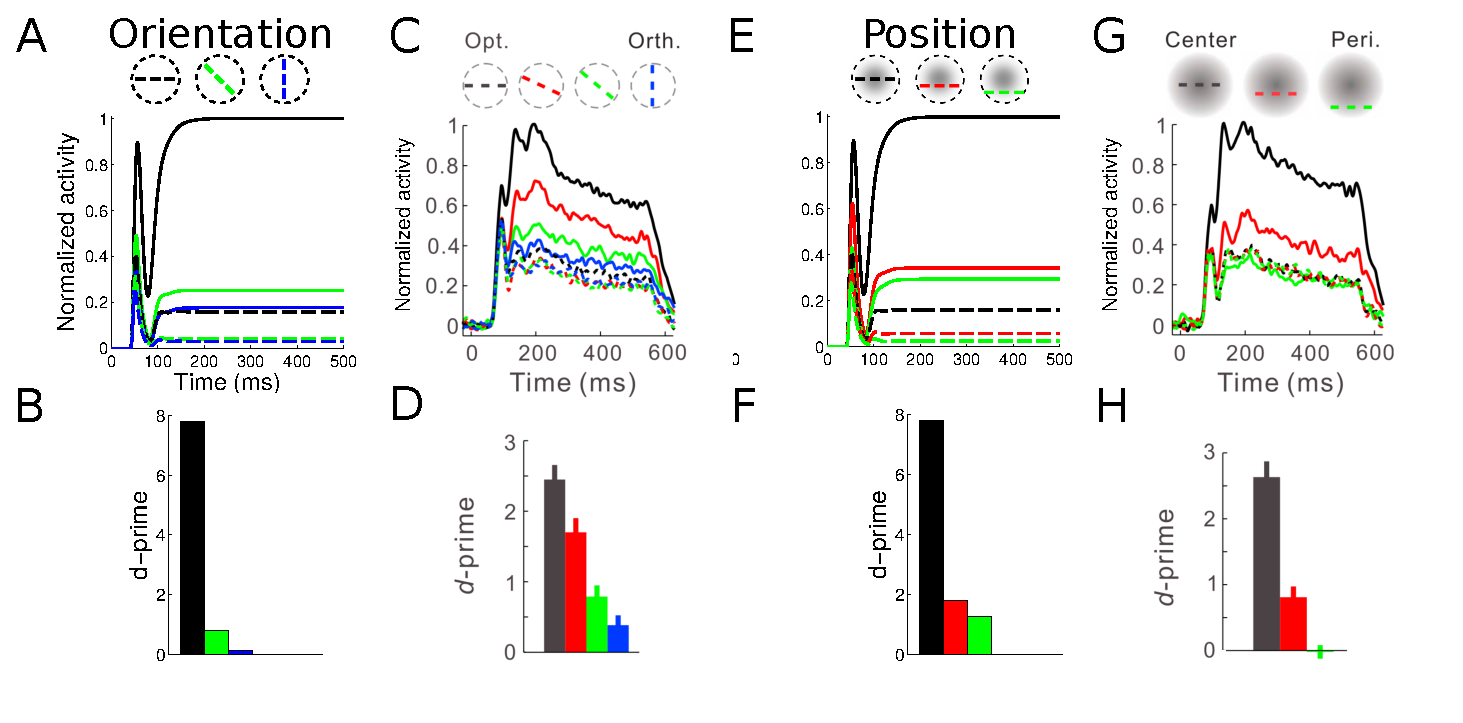
\includegraphics[width=\textwidth]{Contour/figs/FigS1.eps}
\end{center}
\makeatletter
\let\@currsize\normalsize
\caption[Orientation and position dependence of contour integration in V4]{Orientation and position dependence of contour integration in
  V4 $G_c$ cells. The top row shows neuronal responses and the bottom
  row the contour-response $d'$.  Line colors for each figure are
  indicated by the legends at the top of each column. Top row, solid
  lines indicate responses for the 7-bar contour pattern, while dashed
  lines indicate responses for the 1-bar noise pattern.  Note that
  orientations were changed in variable steps based on the tuning
  curve of the neuron under study in the experimental data
  (panels~C,~D) while our simulation only allowed steps of
  $\pi/4$ (panels~A,B).  (A and B) Model results, orientation
  dependence.
 The neuronal responses (A) and the contour-response $d'$
  (B) decreased when the contour was rotated away from the preferred
  orientation. (C and D) Analogous experimental results, adapted from
  \cite{Chen_etal14}.
  (E and F) Model
  results, position dependence.
 The neuronal responses (E) and
  contour-response $d'$ (F) decreased when the contour was translated away from the center of the V4 RF.
  (G and H) Analogous experimental results, adapted from \cite{Chen_etal14}. Panels C, D, G, and H are modified from Figure~3 of~\cite{Chen_etal14}.}
\label{Fig:V4_total}
\end{figure}

\begin{figure}[t]
\begin{center}
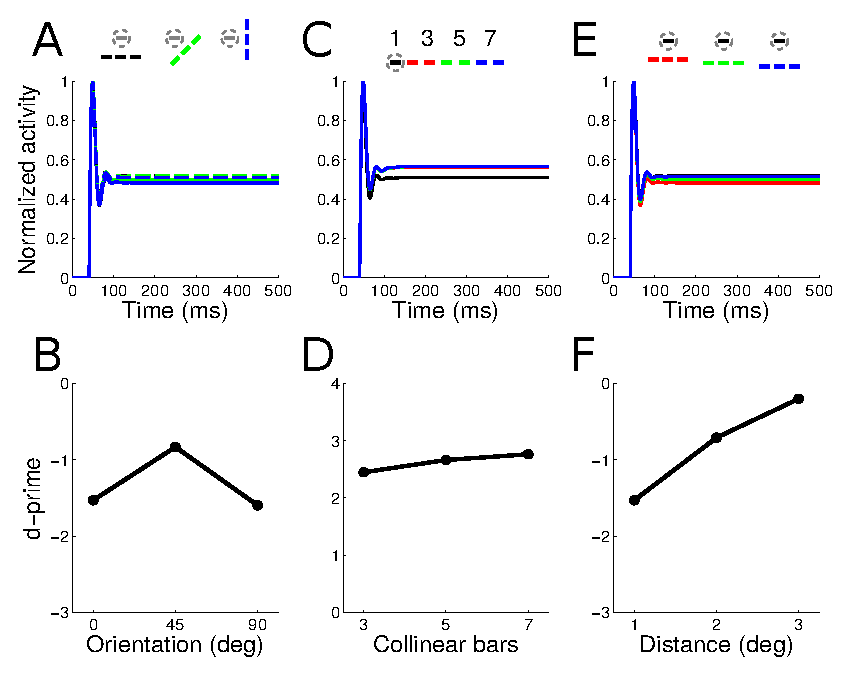
\includegraphics[width=\textwidth]{Contour/figs/FigS2.eps}
\end{center}
\makeatletter
\let\@currsize\normalsize
\caption[Orientation and position dependence of contour integration in V1]{Orientation and position dependence of contour integration in
  V1 $E$ cells, model results. The top row shows neuronal responses
  and the bottom row the contour-response $d'$. Line colors for each
  figures are indicated by the legends at the top of each column. (A
  and B) Orientation dependence of background suppression. The
  neuronal responses (A) and the contour-response $d'$ (B) increased
  for intermediate orientations of the background contour.
  In (A), solid and
  dashed lines correspond to the 7-bar contour and 1-bar noise patterns, respectively.
  (C and D) Contour integration on one end. The neuronal responses (C)
  and contour-response $d'$ (D) increased when bars were added to only
  one side of the V1 RF. (E and F) Position dependence of background
  suppression.  The neuronal responses (E) and contour-response $d'$ (F) increased (approached zero) when the background contour was moved away from the center of the V1 RF.}
\label{Fig:V1_total}
\end{figure}

%%% Local Variables:
%%% mode: latex
%%% TeX-master: "../root"
%%% End:


%% REFERENCES

% if you use BIBTEX
\bibliographystyle{IEEEtran}
\bibliography{thesis}

\begin{vita}

\begin{wrapfigure}{l}{0pt}
\includegraphics[width=2in,height=2.5in,clip,keepaspectratio]{bhh_headshot}
\end{wrapfigure}

Brian H. Hu received the Sc.\ B.\ degree in Bioengineering
from the University of Pittsburgh in May 2011,  and enrolled in the Biomedical Engineering Ph.D.\ program at Johns Hopkins University in August 2011.  He was a recipient of the University Honors College full-tuition scholarship, and also the Swanson School of Engineering Outstanding Senior Award and the Department of Bioengineering Outstanding Student of the Year Award in 2011. His research involves modeling the neural mechanisms of perceptual organization and selective attention, and his papers have been published in Vision Research and Journal of Computational Neuroscience.

% TO DO: What next?
%Starting in June 2007, Jacob will work on the ``Revolutionizing Prosthetics 2009'' 
%project at the Johns Hopkins University Applied Physics Laboratory in Laurel,
%MD, where he will help to create the next-generation of upper-arm
%neuroprostheses.  

\end{vita}
\end{document}
